\cleardoublepage
\chapter{Network}

The problem of transmitting large data is one of the open problems in the information technology research area. A teleoperated system like the one presented in this work needs a stable, low-latency connection with high bandwidth requirements. Ensuring the reliability of communication between different components is crucial, especially in systems where even a brief connection drop could lead to potential malfunctions or pose risks to human safety. In scenarios involving teleoperation, the synchronisation between various data streams must be flawless, requiring both stable network connections and efficient data handling strategies.
\section{Requirements}
In \autoref{tab:connection-requirements:comparison}, we report the connection requirements for the different components of the framework. We define a component as \textit{critical} when a connection drop could harm the patient or cause damage to the equipment. \textit{High bandwidth} refers to a bandwidth need~$>$5MB/s, while \textit{Low latency} refers to latencies~$<$5ms. As we can see, visualisation parts are never critical, while hardware controllers are. It is also worth noting that while the visual components of the system are deemed \textit{non-critical} in terms of connection stability, the clarity and quality of transmitted images can still significantly impact the operator's decision-making process.
%\begin{itemize}
%	\item Ultrasound image stream: high bandwidth with medium latency
%	\item Force/Torque measurement from the F/T sensor: very low bandwidth but also very low latency
%	\item Point cloud of the patient: high bandwidth with medium latency
%	\item leader haptic device target pose: very low bandwidth and very low latency
%	\item SMPL body parameters: very low bandwidth and medium latency
%	content...
%\end{itemize}
\newcommand{\cmark}{\ding{51}}%
\newcommand{\xmark}{\ding{55}}%

\begin{table*}[!ht]
	\centering
	\begin{tabular}{cccc}
            \toprule
		% \hline
		\sc{Component} & \sc{Critical} & \sc{High Bandwidth} & \sc{Low Latency} \\
		% \hline
  %           \hline
        \midrule
		Ultrasound image stream & \xmark & \cmark & \cmark \\
		% \hline
		Force/Torque measurement & \cmark & \xmark & \cmark \\
		% \hline
		Haptic device pose measurement & \cmark & \xmark & \cmark \\
		% \hline
		Point cloud of the patient & \xmark & \cmark & \xmark \\
		% \hline
		SMPL body parameters  & \xmark & \xmark & \cmark \\
		% \hline
		Robot state & \xmark & \xmark & \cmark \\
		% \hline
        \bottomrule
	\end{tabular}
	\caption{Connection requirements for the teleoperation framework}
	\label{tab:connection-requirements:comparison}
\end{table*}

\section{Leader-Follower connection}
Since the leader and the follower are not in the same location, a cabled connection between the two is needed to ensure the exchange of information. The middleware used for the communication is ROS2, which already occupies for the information exchange with the well-known topic-subscriber method. ROS2 uses a DDS (data distribution service) to automatically discover new publisher of certain data if they are under the same network. The problem arises when leader and follower are not under the same local network, because different nodes would not be able to conversate.
\section{Husarnet: a ROS2 VPN}
Without the need to modify or rewrite the DDS logic, it is possible to simulate the local network relying on a VPN. Husarnet~\cite{nowak2024husarnet} is a possibility in this sense. It has specific features for ROS2, and it was easy to set up.
After installing the software, each computer can join a Husarnet network with one command. There is also the support for different DDS like \verb*|FastDDS|~(default) and \verb*|CycloneDDS|. An illustrative image showing the purpose is presented in \autoref{fig:connection-requirements:husarnet}.
\begin{figure}[h]
	\centering
	\subfloat[\centering Two hosts cannot communicate using ROS2 DDS even though they are connected. ]{{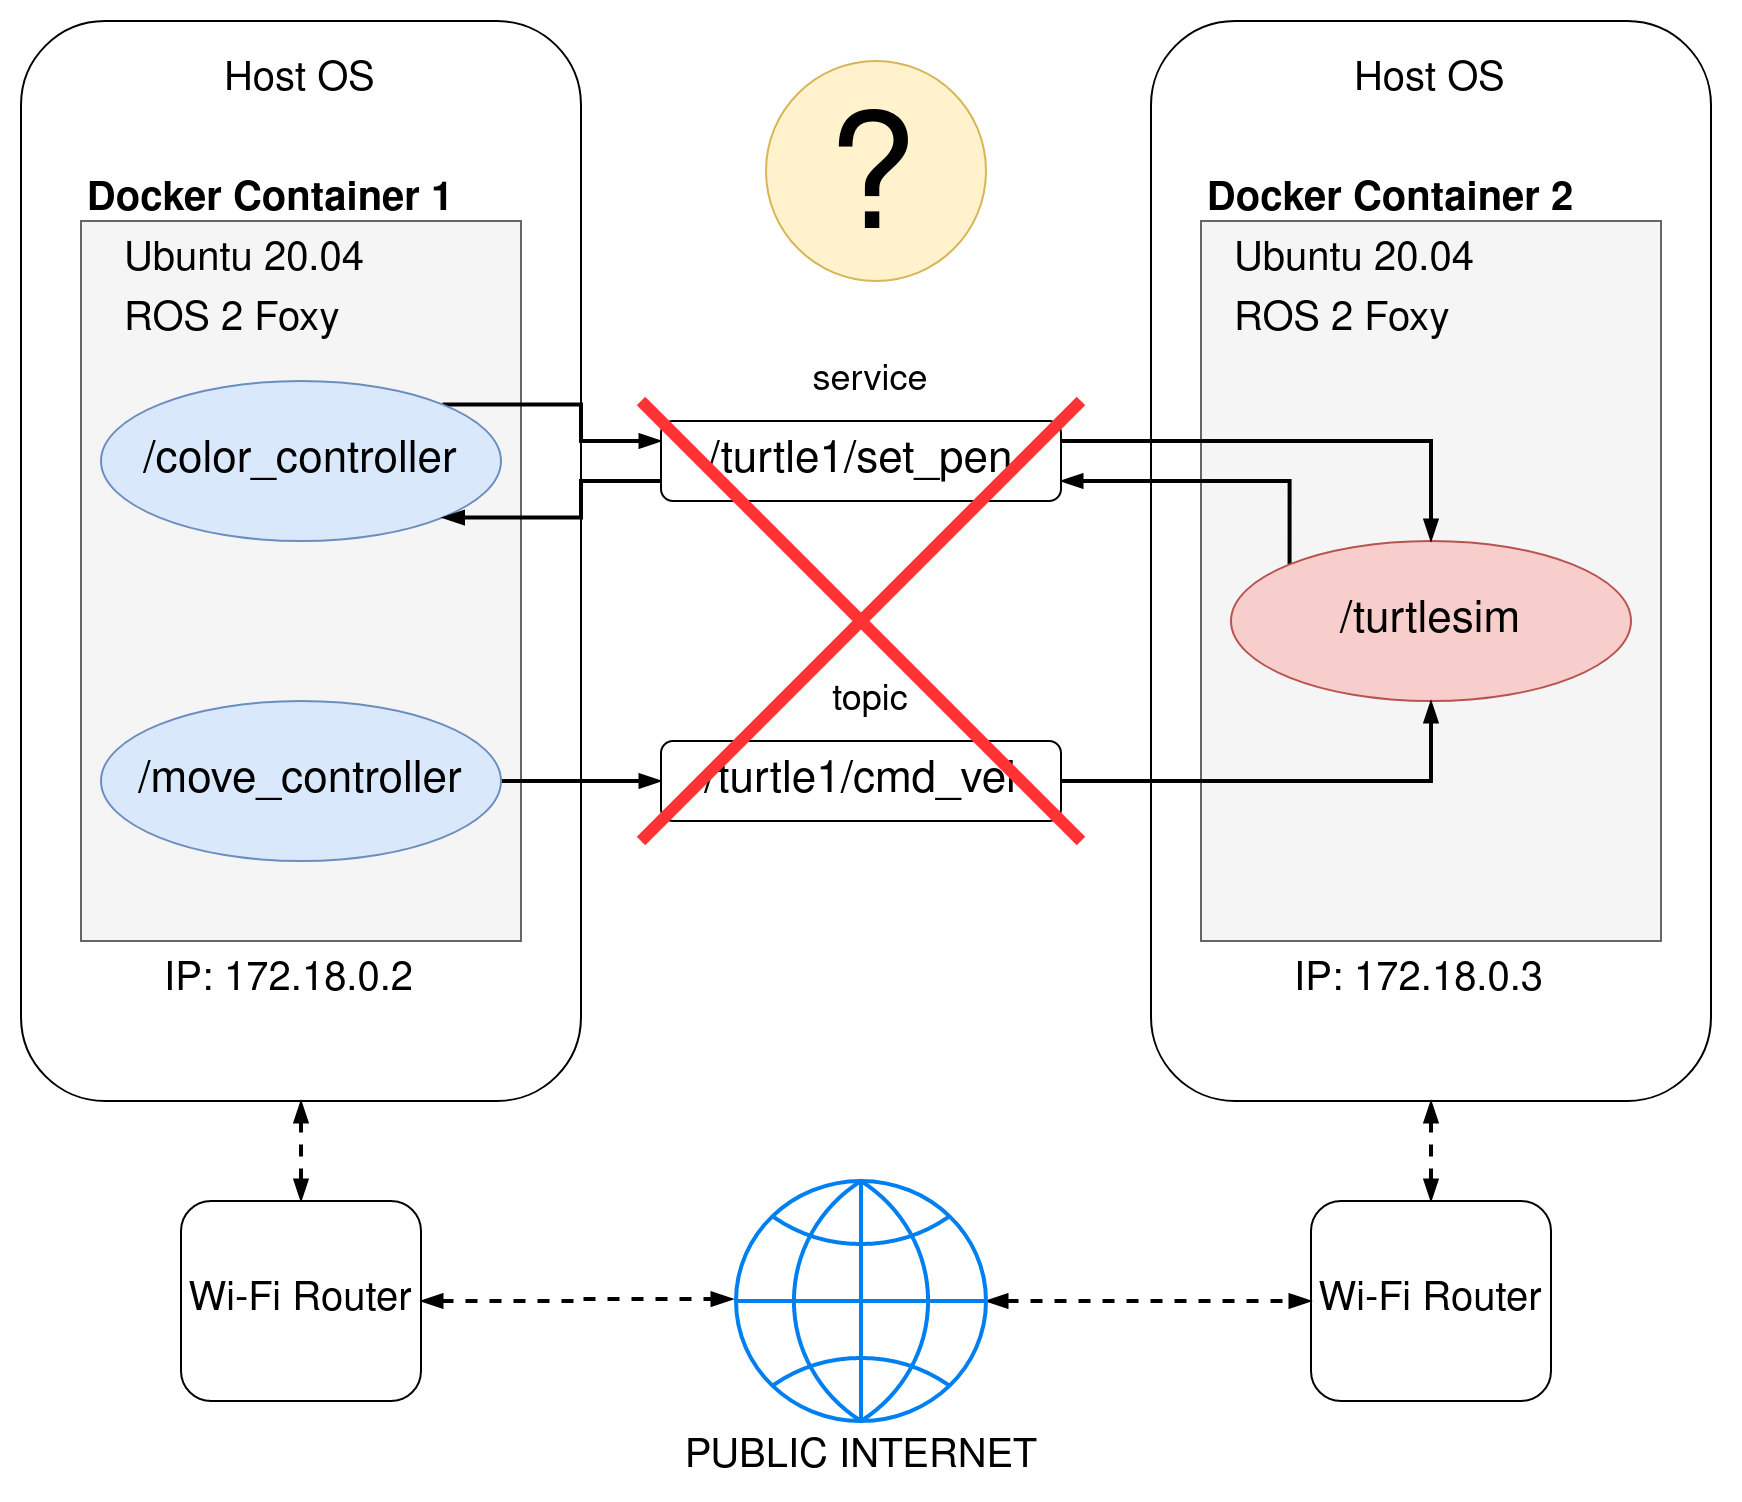
\includegraphics[width=6cm]{images/connection_requirements/husarnet1.png} }}%
	\qquad
	\subfloat[\centering Two hosts can communicate through the Husarnet VPN. ]{{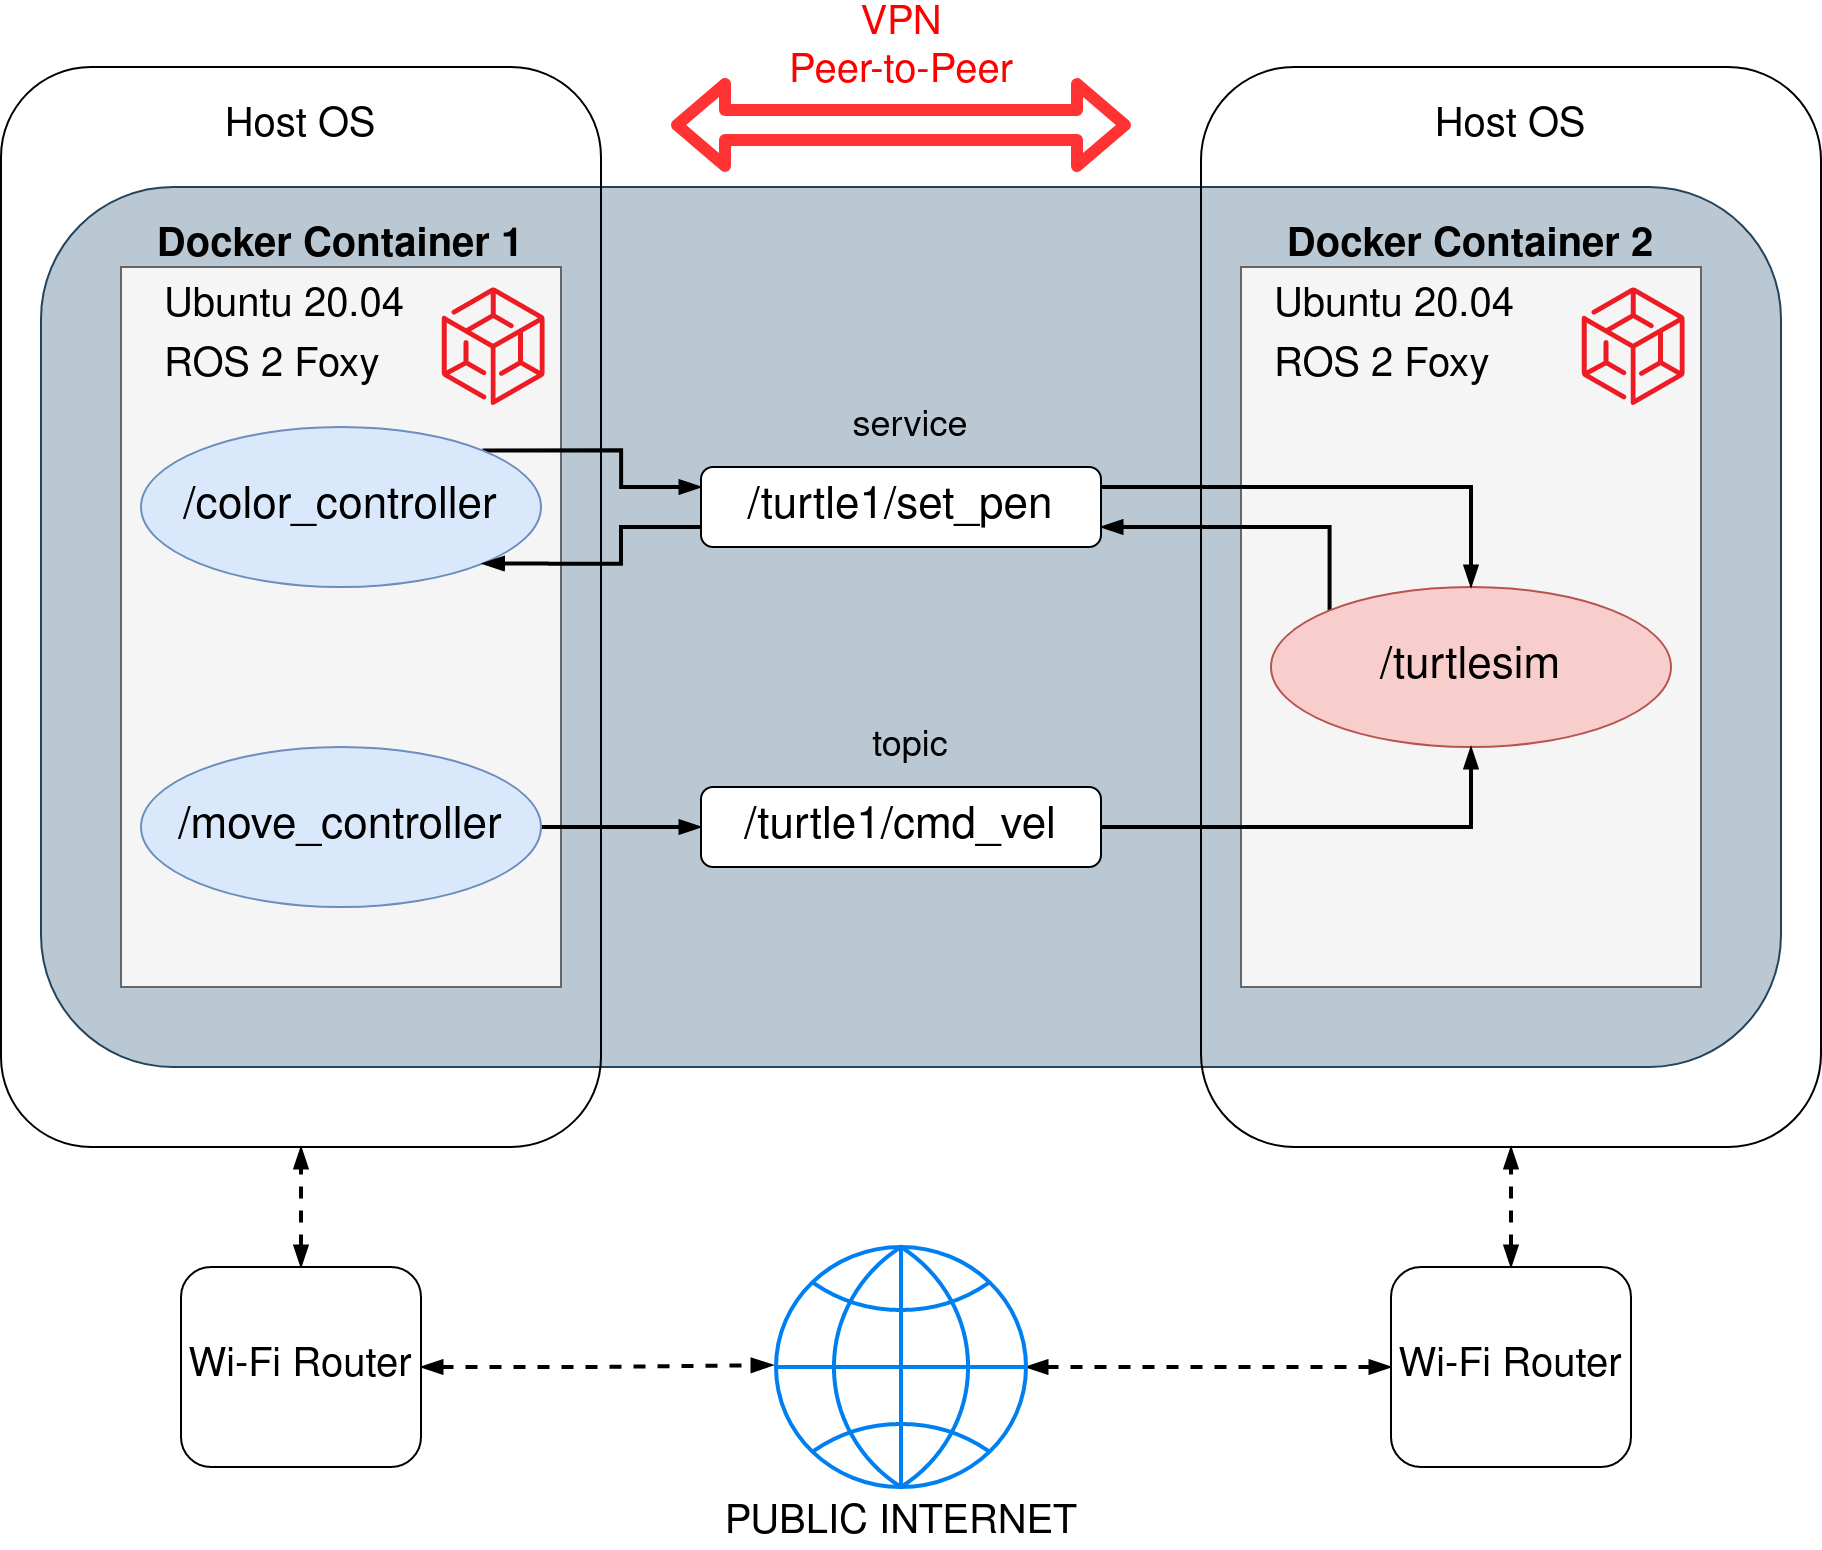
\includegraphics[width=6cm]{images/connection_requirements/husarnet2.png} }}%
	\caption{The Husarnet use scope 
        \label{fig:connection-requirements:husarnet}
 \cite{nowak2024husarnet}}
\end{figure}
As described, the VPN enables peer-to-peer topics and services communication from remote hosts.
In our case, it was sufficient to create a Husarnet network and join that network with both the follower and leader computers. Each computer was given a local IPv6 IP address that is used to broadcast the messages between the two stations.
\section{Compression Algorithms}
To limit the amount of bandwidth used by the RGB image and the point cloud, some algorithms were employed. 
\subsection{Image encoding}
The RGB image is acquired in FHD ($1920x1080$ @$30$FPS) and compressed using \verb|ffmpeg| with \verb|hevc|~(High Efficiency Video Coding a.k.a. H.265) as the encoding. The decision to use HEVC for image encoding stems from its ability to maintain high visual quality while significantly reducing file sizes. This is particularly useful in teleoperation, where the system must handle a continuous flow of data without overwhelming the available bandwidth. This encoding can also leverage on GPU acceleration to speed up coding and decoding of images and videos using \verb|NVENC|~(Nvidia Encoder) thus reducing the feedback delay. The follower encodes the image captured by the \verb|Realsense435| using \verb|hevc_nvenc|, then the compressed image is added to a ROS2 image compressed message and sent to the leader, which decompresses it and renders the result on screen.
\subsection{Point Cloud encoding}
Point cloud data presents a unique challenge due to its inherently large size and complex structure. However, by using the \verb|Draco|~\cite{frank2024Draco} compression algorithm, we are able to significantly reduce the amount of data that needs to be transmitted, without sacrificing the detail and accuracy required for precise teleoperation.
The Draco Algorithm is a CPU-based geometry compression method designed by \verb|Google| to efficiently compress 3D graphics, specifically point clouds and 3D meshes. It reduces the size of large datasets while maintaining high fidelity, making it ideal for our applications. Draco achieves this by encoding vertex positions, connectivity data, colours, normals, and other attributes using techniques like predictive coding and quantisation, significantly reducing the bandwidth required for storage and transmission of 3D models without noticeable loss in visual quality.
The point cloud measured by the \verb|Realsense435| is computed with a depth module profile of $1280x720$@$30$FPS and is compressed using \verb|Draco| in the follower side. Then the compressed data is added to a ROS2 \verb|PointCloud2| message and published to the leader, which can visualise it in VR or through the GUI.